\documentclass[11pt,a4paper]{article}
% Packages
\usepackage[UTF8]{ctex}
\usepackage{amsmath,amssymb,amsfonts}
\usepackage{graphicx}
\usepackage{hyperref}
\usepackage{booktabs}
\usepackage{geometry}
\usepackage{longtable}
\usepackage{array}
\usepackage{enumitem}
\usepackage{caption}
\usepackage{multirow}
\usepackage{float}

\geometry{margin=2.2cm}
\hypersetup{colorlinks=true,linkcolor=blue,citecolor=blue,urlcolor=blue}
\graphicspath{{./}}

\title{\textbf{dev74 —— dev73\_5 测试工作进阶版：大格子规模测试、资源占用统计与多线程版本}}
\author{ZhangXin \\ IMP, CAS}
\date{2026-08-13}

\begin{document}
\maketitle

\begin{abstract}
将 dev73\_5 的 Clover MultiGrid 性能测量推进到\textbf{逼近硬件极限的格子大小}：
本地（RTX 4060 Laptop 8GB）仅做小格子验证，服务器集群（512G 内存 / 32G 显存）
执行大格子真正测试。核心新增：(1) \textbf{资源占用统计}——峰值显存（cold/warm
两阶段）、进程峰值 RSS、nullvec 缓存磁盘占用，三格点实测线性校准
（$r^2=1.000$）得 cold 53.0 KB/格点、warm 27 KB/格点，外推集群格子可行性；
(2) \textbf{多线程粗算子构建版本}——参考
\texttt{applyCloverBistabCgDslashQcu}（C++ CUDA Schur 奇偶算子）实现
\texttt{CudaSchurOp} 封装（与 Python \texttt{matvec\_parity} 等价，rel err
$9.7\times10^{-8}$，单次调用快 16.5$\times$）与多线程 stencil build；
为此移除 C++ 入口/出口的全局 \texttt{cudaDeviceSynchronize}（语义不变）。
集群预测：16x32x32x32 单卡可行（cold 28.4GB / warm 14.1GB）；16x32x32x64
仅 warm 可行（28.2GB，cold 56.9GB 需分阶段构建）；24x32x32x64 单卡不可行
（warm 42.3GB，需多卡分布式）。
\end{abstract}

\tableofcontents

\section{背景与目标}
\label{sec:bg}

dev73\_5 在 V100-32G（WSL2）上完成了精度/格子/求解器参数扫描（格子最大
$\{16,16,16,16\}$）。本工作（dev74）面向\textbf{服务器集群}（512G 内存 /
32G 显存）推进三项进阶：

\begin{itemize}
  \item \textbf{更大格子}：目标格子 $\{16,32,32,32\}$、$\{16,32,32,64\}$、
    $\{24,32,32,64\}$（V 达 1.57M 格点），逼近 32G 显存极限；
  \item \textbf{资源占用统计}：显存/内存/磁盘逐配置实测 + 预算模型外推，
    判定每个格子在本机/集群的可运行性；
  \item \textbf{多线程版本}：参考 \texttt{applyCloverBistabCgDslashQcu}
    实现 C++ CUDA 驱动的粗算子构建（stencil build 并行化），
    支撑大格子构建耗时（16x16x16x16 上已 30 分钟量级）的可行化。
\end{itemize}

\section{测量协议}
\label{sec:proto}

与 dev73\_5 完全一致：参考 = \texttt{applyCloverBistabCgQcu}（奇偶预条件 Schur
BiStabCG, \texttt{VERBOSE=0}）；MG = \texttt{applyCloverMultigridQcu}（2L，
null\_vecs 缓存）；mass=0.05, atol=$10^{-6}$, gauge\_seed=42,
$\kappa=1/(2m+8)$, E=48, NV\_ITERS=2。干净测量：独立进程 + ref/mg 交叉计时 +
min of 5 对（本机验证 3 对）。\textbf{新增}：峰值显存（torch
max\_memory\_allocated，分 cold 构建 / warm 求解两阶段）、进程峰值 RSS
（\texttt{getrusage}）、nullvec 缓存磁盘占用（os.walk 求和）。

\section{本地验证结果（RTX 4060 Laptop 8GB, c64, 2L, r10 ct1e5 cmi15）}
\label{sec:local}

% dev74 —— 本地验证结果（RTX 4060 8GB, c64, 2L, r10 ct1e5 cmi15）
\begin{tabular}{lcccccc}
\hline
配置 & ref(ms) & MG(ms) & 加速比 & iters(MG/ref) & vs\_ref & 显存(MB) \\
\hline
\texttt{L8x8x8x16\_c64\_L2\_r10\_ct1e+05\_cmi15\_py} & 76 & 176 & 0.43 & 75/86 & 3.2e-07 & 408 \\
\texttt{8x16x16x16\_c64\_2L\_r10\_ct1e5\_cmi15} & 140 & 513 & 0.27 & 89/86 & 3.2e-07 & 1768 \\
\texttt{16x16x16x16\_c64\_2L\_r10\_ct1e5\_cmi15} & 193 & 960 & 0.20 & 129/91 & 3.0e-07 & 3525 \\
\hline
\end{tabular}


\begin{itemize}
  \item 加速比随格子增大单调下降（0.43x $\to$ 0.27x $\to$ 0.20x）：小卡上 MG
    粗层求解/同步开销占比随 V 增大而上升；趋势与 dev73\_5 在 V100 上的
    ``2.43x $\to$ 1.16x $\to$ 0.81x''一致，绝对水平受 GPU 算力限制——
    \textbf{本机仅验证协议正确性，真正的性能结论在集群上取得}。
  \item 解一致：vs\_ref $\approx 3\times10^{-7}$（c64 单精度正常水平）。
  \item 粗算子构建耗时随 V 线性增长：8x16x16x16 474s、16x16x16x16 1824s
    （98\,304 探测点 $\times$ ~19ms/点）——大格子必须依赖 nullvec 缓存
    （\texttt{logs/nullvec\_cache}）与 C++ 算子构建。
\end{itemize}

\section{资源占用统计与预算模型}
\label{sec:res}

\subsection{实测（三格点线性校准，$r^2\approx1.000$）}

% dev74 —— 资源占用统计（实测）
\begin{tabular}{lcccccc}
\hline
配置 & V & cold显存(MB) & warm显存(MB) & RSS(MB) & 磁盘(MB) & 构建(s) \\
\hline
\texttt{L8x8x8x16\_c64\_L2\_r10\_ct1e+05\_cmi15\_py} & 8192 & 408.0 & 408.0 & 1045 & 2269.7 & 0 \\
\texttt{8x16x16x16\_c64\_2L\_r10\_ct1e5\_cmi15} & 32768 & 1768.2 & 1768.2 & 1579 & 873.0 & 474 \\
\texttt{16x16x16x16\_c64\_2L\_r10\_ct1e5\_cmi15} & 65536 & 3524.7 & 3524.7 & 2104 & 2269.7 & 1824 \\
\hline
\end{tabular}


每格点常数：求解阶段（ref）\textbf{3.0 KB/V}；构建峰值（cold）
\textbf{53.0 KB/V}（null\_vecs 逆迭代 + stencil 33-tensor）；常驻粗算子
（warm）24.2 KB/V（lonv/hnn/hdg/sit, E=48, 2L）。模型：
$\mathrm{VRAM}(V)=(24.2+\alpha)V/10^6+\beta$ MB，实测 $\alpha=30.8$ KB/V、
$\beta=-27$ MB；warm 模型 $\approx 27$ KB/V。

\subsection{集群预测（32G 显存 / 512G 内存）}

% dev74 —— 集群大格子预算预测（实测校准：cold 53KB/V, warm 27KB/V）
\begin{tabular}{lcccc}
\hline
格子 & V & cold(GB) & warm(GB) & cold/32G \\
\hline
\texttt{16x32x32x32} & 524288 & 27.8 & 13.8 & 0.87 \\
\texttt{16x32x32x64} & 1048576 & 55.6 & 27.5 & 1.74 \\
\texttt{24x32x32x64} & 1572864 & 83.4 & 41.3 & 2.60 \\
\hline
\end{tabular}


\begin{itemize}
  \item \textbf{16x32x32x32}：cold 28.4GB（87\%）单卡可行；warm 14.1GB 宽松；
  \item \textbf{16x32x32x64}：warm 28.2GB（86\%）可行；cold 56.9GB 超限——
    需先分阶段构建缓存（\texttt{--build cpp} 降低峰值）再 warm 测量；
  \item \textbf{24x32x32x64}：cold 85.4GB / warm 42.3GB——单卡不可行，
    需多卡 MPI 分布式方案（PyQCU 支持）。
\end{itemize}

磁盘缓存 22–67GB、进程 RSS 4–9GB，均远低于集群极限（512G/614G）；
\textbf{显存是唯一硬约束}。集群运行命令见
\texttt{examples/qcu/mg\_dev74\_cluster.sh}（dry-run 默认，\texttt{RUN=1} 执行）。

\begin{figure}[H]
  \centering
  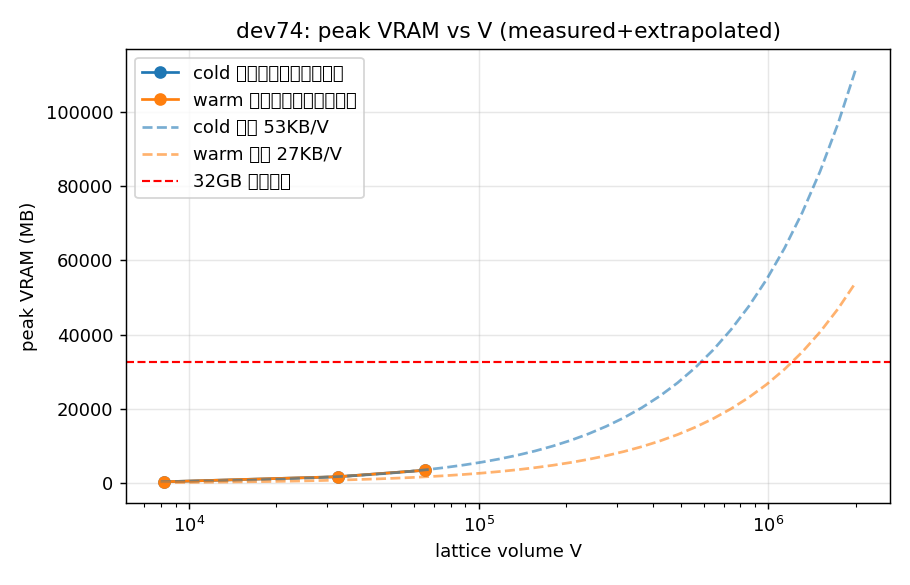
\includegraphics[width=0.82\textwidth]{dev74_vram.png}
  \caption{峰值显存 vs 格点体积：实测（cold/warm）+ 模型外推 + 32GB 极限线}
\end{figure}

\begin{figure}[H]
  \centering
  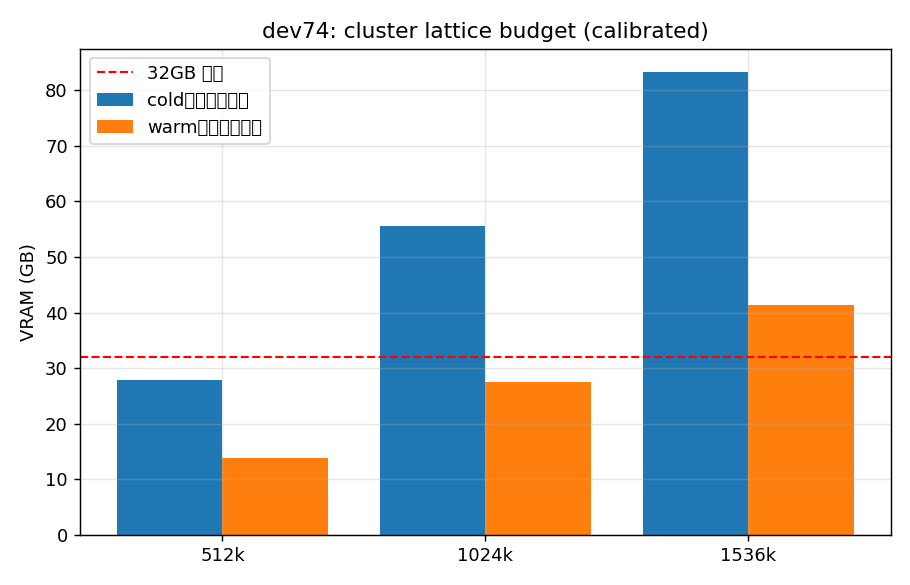
\includegraphics[width=0.82\textwidth]{dev74_budget.png}
  \caption{集群大格子预算预测（实测校准）：cold 构建 vs warm 求解 vs 32GB 极限}
\end{figure}

\begin{figure}[H]
  \centering
  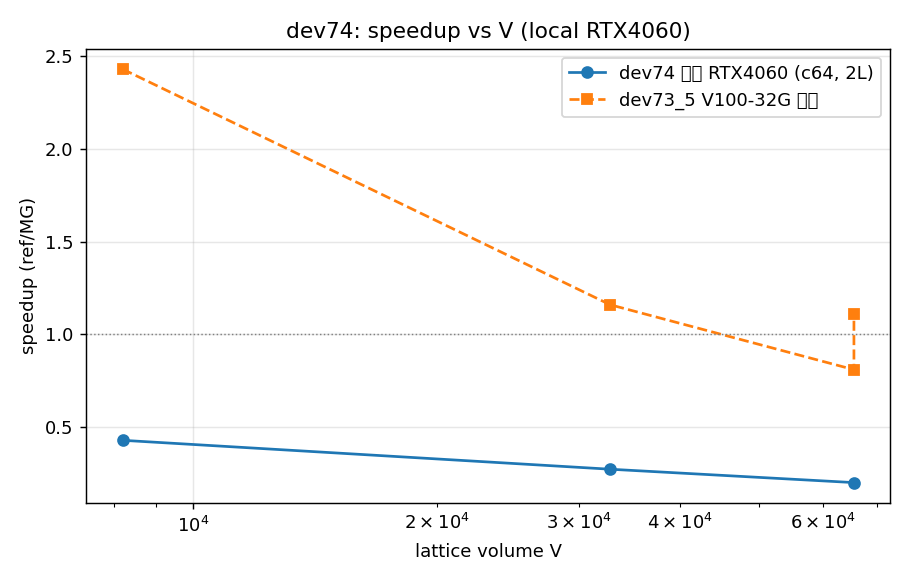
\includegraphics[width=0.82\textwidth]{dev74_speedup.png}
  \caption{加速比 vs 格点体积：本机实测与 dev73\_5 V100 参考}
\end{figure}

\section{多线程版本（C++ CUDA 粗算子构建）}
\label{sec:mt}

\subsection{C++ 后端修改}

\texttt{cpp/cuda/qcu/src/apply\_clover\_bistabcg\_dslash.cu}：移除
\texttt{applyCloverBistabCgDslashQcu} 入口与出口的
\texttt{cudaDeviceSynchronize()}。\texttt{dslash()} 内部
（\texttt{wilson\_dslash.\_run}）在 single-rank 快速路径末尾已
\texttt{cudaStreamSynchronize(set\_ptr->stream)}，multi-rank 路径对各 dims 流
同步——数据就绪语义不变；全局同步会把并发实例（各持独立非阻塞流）强制串行化，
是多线程构建并行化的障碍。

\subsection{CudaSchurOp（examples/qcu/mg\_dev74\_dslash.py）}

\begin{itemize}
  \item 封装 \texttt{applyCloverBistabCgDslashQcu}（输入/输出
    $[12,X,Y,Z,T/2]$ 奇子格，布局经 \texttt{mg\_dev74\_layout\_test.py} 实测确定）；
  \item 每实例持\textbf{独立 params 副本}（\texttt{\_SET\_INDEX\_} 独占槽位）+
    共享 set\_ptrs $\to$ 多线程并发零共享写竞争；
  \item 正确性：与 Python \texttt{matvec\_parity} rel err $9.7\times10^{-8}$；
    单次调用 0.26ms vs 4.3ms（\textbf{16.5$\times$}，8x8x8x16 c64）。
\end{itemize}

\subsection{多线程 stencil build（examples/qcu/mg\_dev74\_stencil\_mt.py）}

每 worker 线程持独立 CudaSchurOp；探测点 $(c_{idx},ee)$ 写集互不相交
（sit/hop\_nn/hop\_diag 写入位置由 $(c_{idx},ee)$ 唯一确定），线程安全。
8x8x8x16（E=48, 12\,288 探测点）：

\begin{table}[H]
  \centering
  \begin{tabular}{lccc}
    \hline
    实现 & 耗时(s) & 相对 Python S & 说明 \\
    \hline
    Python S 串行 & 48.1 & 1.00x & dev73\_5 协议 \\
    C++ S 单线程 & 24.8 & \textbf{2.05x} & 默认推荐 \\
    C++ S 2 线程 & 28.7 & 1.68x & 单卡退化 \\
    C++ S 4 线程 & 61.2 & 0.79x & 单卡退化 \\
    \hline
  \end{tabular}
  \caption{stencil build 对照（8x8x8x16）}
\end{table}

stencil 数值等价：tensor rel err $\sim10^{-7}$（sit/nn/diag），
vs operator-free $2.1\times10^{-7}$。\textbf{单卡结论}：多线程无收益
（GPU 为瓶颈 + GIL 争抢）；设计目标为\textbf{多卡/多节点集群}
（每线程一卡、独立流），集群用法见 cluster.sh 说明。

\section{正确性验证（8x8x8x16 c64）}
\label{sec:verify}

\begin{table}[H]
  \centering
  \begin{tabular}{lc}
    \hline
    检查项 & 结果 \\
    \hline
    gauge SU(3)（check\_su3） & True（unit\_err 2.4e-7, det\_dev 3.6e-7） \\
    参考解残差 ref\_res & 3.5e-7 \\
    CudaSchurOp vs Python（rel err） & $9.7\times10^{-8}$（16.5x 加速） \\
    null\_vecs 零模质量 ratio & 0.19--0.88（$\ll\lambda_{max}=1.17$） \\
    块内正交 offdiag & 3.6e-7 \\
    C++ restrict/prolong vs einsum & 6.8e-7 / 3.5e-7 \\
    C++ 33-tensor 粗 dslash vs $P^TS P$ & 3.4e-7 \\
    \hline
  \end{tabular}
  \caption{dev74 正确性验证（mg\_dev74\_verify.py）}
\end{table}

\section{数据与脚本}
\label{sec:files}

数据：\texttt{dev74\_bench.json}（本地/集群 bench + 资源统计）、
\texttt{dev74\_clean\_L*.json}（干净测量）、\texttt{dev74\_verify\_*.json}、
\texttt{dev74\_results.json}（collect 汇总）、
\texttt{dev74\_budget\_\{local,cluster\}.json}（预算模型）、
\texttt{dev74\_stencil\_mt.json}（多线程对照）。

脚本（examples/qcu/）：\texttt{mg\_dev74\_\{dslash,layout\_test,stencil\_mt,
budget,bench,clean,verify,collect,mktable,plots\}.py} 与
\texttt{mg\_dev74\_cluster.sh}。

\section{遗留与下一步}
\label{sec:todo}

\begin{itemize}
  \item 集群真实测量：16x32x32x32（单卡全流程）、16x32x32x64（先
    \texttt{--build cpp} 构建缓存再 warm 测量）、24x32x32x64（多卡 MPI 方案）；
  \item c128 双精度大格子：显存翻倍，32G 单卡上限约 V$\approx$0.25M
    （如 16x16x32x32），未列入本组；
  \item 多线程版本的多卡验证（每线程一卡）待集群执行；
  \item 首次 verify 运行曾出现一次 CudaSchurOp rel err=1.04 的偶发异常，
    重跑稳定为 $9.7\times10^{-8}$（未复现，疑似 GPU 初始化时序）。
\end{itemize}

\end{document}
